% ============================================================
%  ISEE 2026 — One-Page Abstract
%  International Symposium on Energy & Environment
%  RUET Auditorium, Thursday 20 August 2026
% ============================================================

\documentclass[10pt, a4paper]{article}

% ---------- Packages ----------
\usepackage[
  top=0.85cm, bottom=0.85cm,
  left=1.9cm, right=1.9cm
]{geometry}
\usepackage{times}
\usepackage[T1]{fontenc}
\usepackage[utf8]{inputenc}
\usepackage{amsmath}
\usepackage{graphicx}
\usepackage{booktabs}
\usepackage{array}
\usepackage{xcolor}
\usepackage{hyperref}
\usepackage{microtype}
\usepackage{caption}
\usepackage{parskip}
\usepackage{float}

% ---------- Hyperlink style ----------
\hypersetup{
  colorlinks = true,
  urlcolor   = blue,
  linkcolor  = black,
  citecolor  = black
}

% ---------- Caption setup ----------
\captionsetup{font=footnotesize, labelfont=bf, skip=1pt}

% ---------- Spacing ----------
\setlength{\parindent}{0pt}
\setlength{\parskip}{0.5pt}
\setlength{\intextsep}{1pt}
\setlength{\textfloatsep}{2pt}
\setlength{\floatsep}{2pt}
\setlength{\abovecaptionskip}{1pt}
\setlength{\belowcaptionskip}{0pt}
\setlength{\aboverulesep}{0.15ex}
\setlength{\belowrulesep}{0.25ex}

% ============================================================
\begin{document}
\linespread{0.96}\selectfont

% [All Times New Roman, 10 pts]

% ---------- TITLE ----------
\begin{center}
  {\fontsize{12}{14}\selectfont\bfseries
  Green V2X: An Energy-Aware Handoff Strategy for Reducing\\[0.5pt]
  Uplink Transmission Energy and CO\textsubscript{2} Emissions\\[0.5pt]
  in Vehicular Networks}
\end{center}

\vspace{1pt}

% ---------- AUTHOR ----------
\begin{center}
  {\fontsize{10}{12}\selectfont
  Ranesh Das Rik\textsuperscript{1,\,*}
  }
\end{center}

\vspace{1pt}

% ---------- AFFILIATION ----------
\begin{center}
  {\fontsize{9}{11}\selectfont
  \textsuperscript{1}Department of Electronics \& Telecommunication Engineering,
  Rajshahi University of Engineering \& Technology, Rajshahi-6204\\[1pt]
  Presenting Author: \href{mailto:rik.ete51@gmail.com}{rik.ete51@gmail.com}
  \quad *Corresponding Author: \href{mailto:rik.ete51@gmail.com}{rik.ete51@gmail.com}
  }
\end{center}

\vspace{2pt}
\hrule
\vspace{2pt}

% ---------- ABSTRACT BODY ----------
\noindent\textbf{Abstract:}

Vehicle-to-Everything (V2X) communication is central to next-generation intelligent
transportation systems, where moving vehicles continuously maintain uplink connections
with roadside cellular base stations (BSs). As a vehicle traverses a highway, it must
periodically switch its serving BS --- a process known as \textit{handoff}. Conventional
handoff policies select the BS with the strongest received signal strength indicator (RSSI)
or highest signal-to-interference-plus-noise ratio (SINR), with no regard for the energy
cost of the chosen radio link. This energy-blind approach leads to avoidable transmit power
expenditure and unnecessary CO\textsubscript{2} emissions --- a growing concern as
vehicular networks scale toward millions of connected vehicles worldwide.

This work presents \textbf{Green V2X}, a research simulation framework that introduces and
evaluates an \textbf{Energy-Aware Handoff (EAH)} algorithm for highway V2X uplink scenarios.
The EAH algorithm scores each candidate BS using a composite metric that minimises
\textit{Energy Per Bit} (EPB) --- joules consumed per bit successfully delivered --- while
jointly accounting for BS load (preferring under-utilised cells), Quality-of-Service (QoS)
constraints (minimum data rate and SINR thresholds), and a cell-edge stability penalty.
Switching decisions employ hysteresis with a time-to-trigger (TTT) timer and per-vehicle
cooldown periods to suppress ping-pong oscillations; forced-trigger rules override hysteresis
when the current BS is severely overloaded or the link degrades beyond acceptable bounds.
The simulator models realistic highway mobility (multi-lane, lane-dependent speeds, stochastic
lane changes), a full physical-layer channel (path loss, weather attenuation, shadowing, fast
fading, inter-cell interference), a PA-level energy model, and a CO\textsubscript{2}
conversion pipeline calibrated to the Bangladesh electricity grid carbon intensity.
Seven classical and literature-inspired baseline algorithms are benchmarked under identical,
seed-controlled conditions for a rigorous and fair comparison.

% ---------- FIGURE + TABLE (side-by-side, one page) ----------
\begin{figure}[H]
  \centering
  \begin{minipage}[t]{0.5\linewidth}
    \centering
    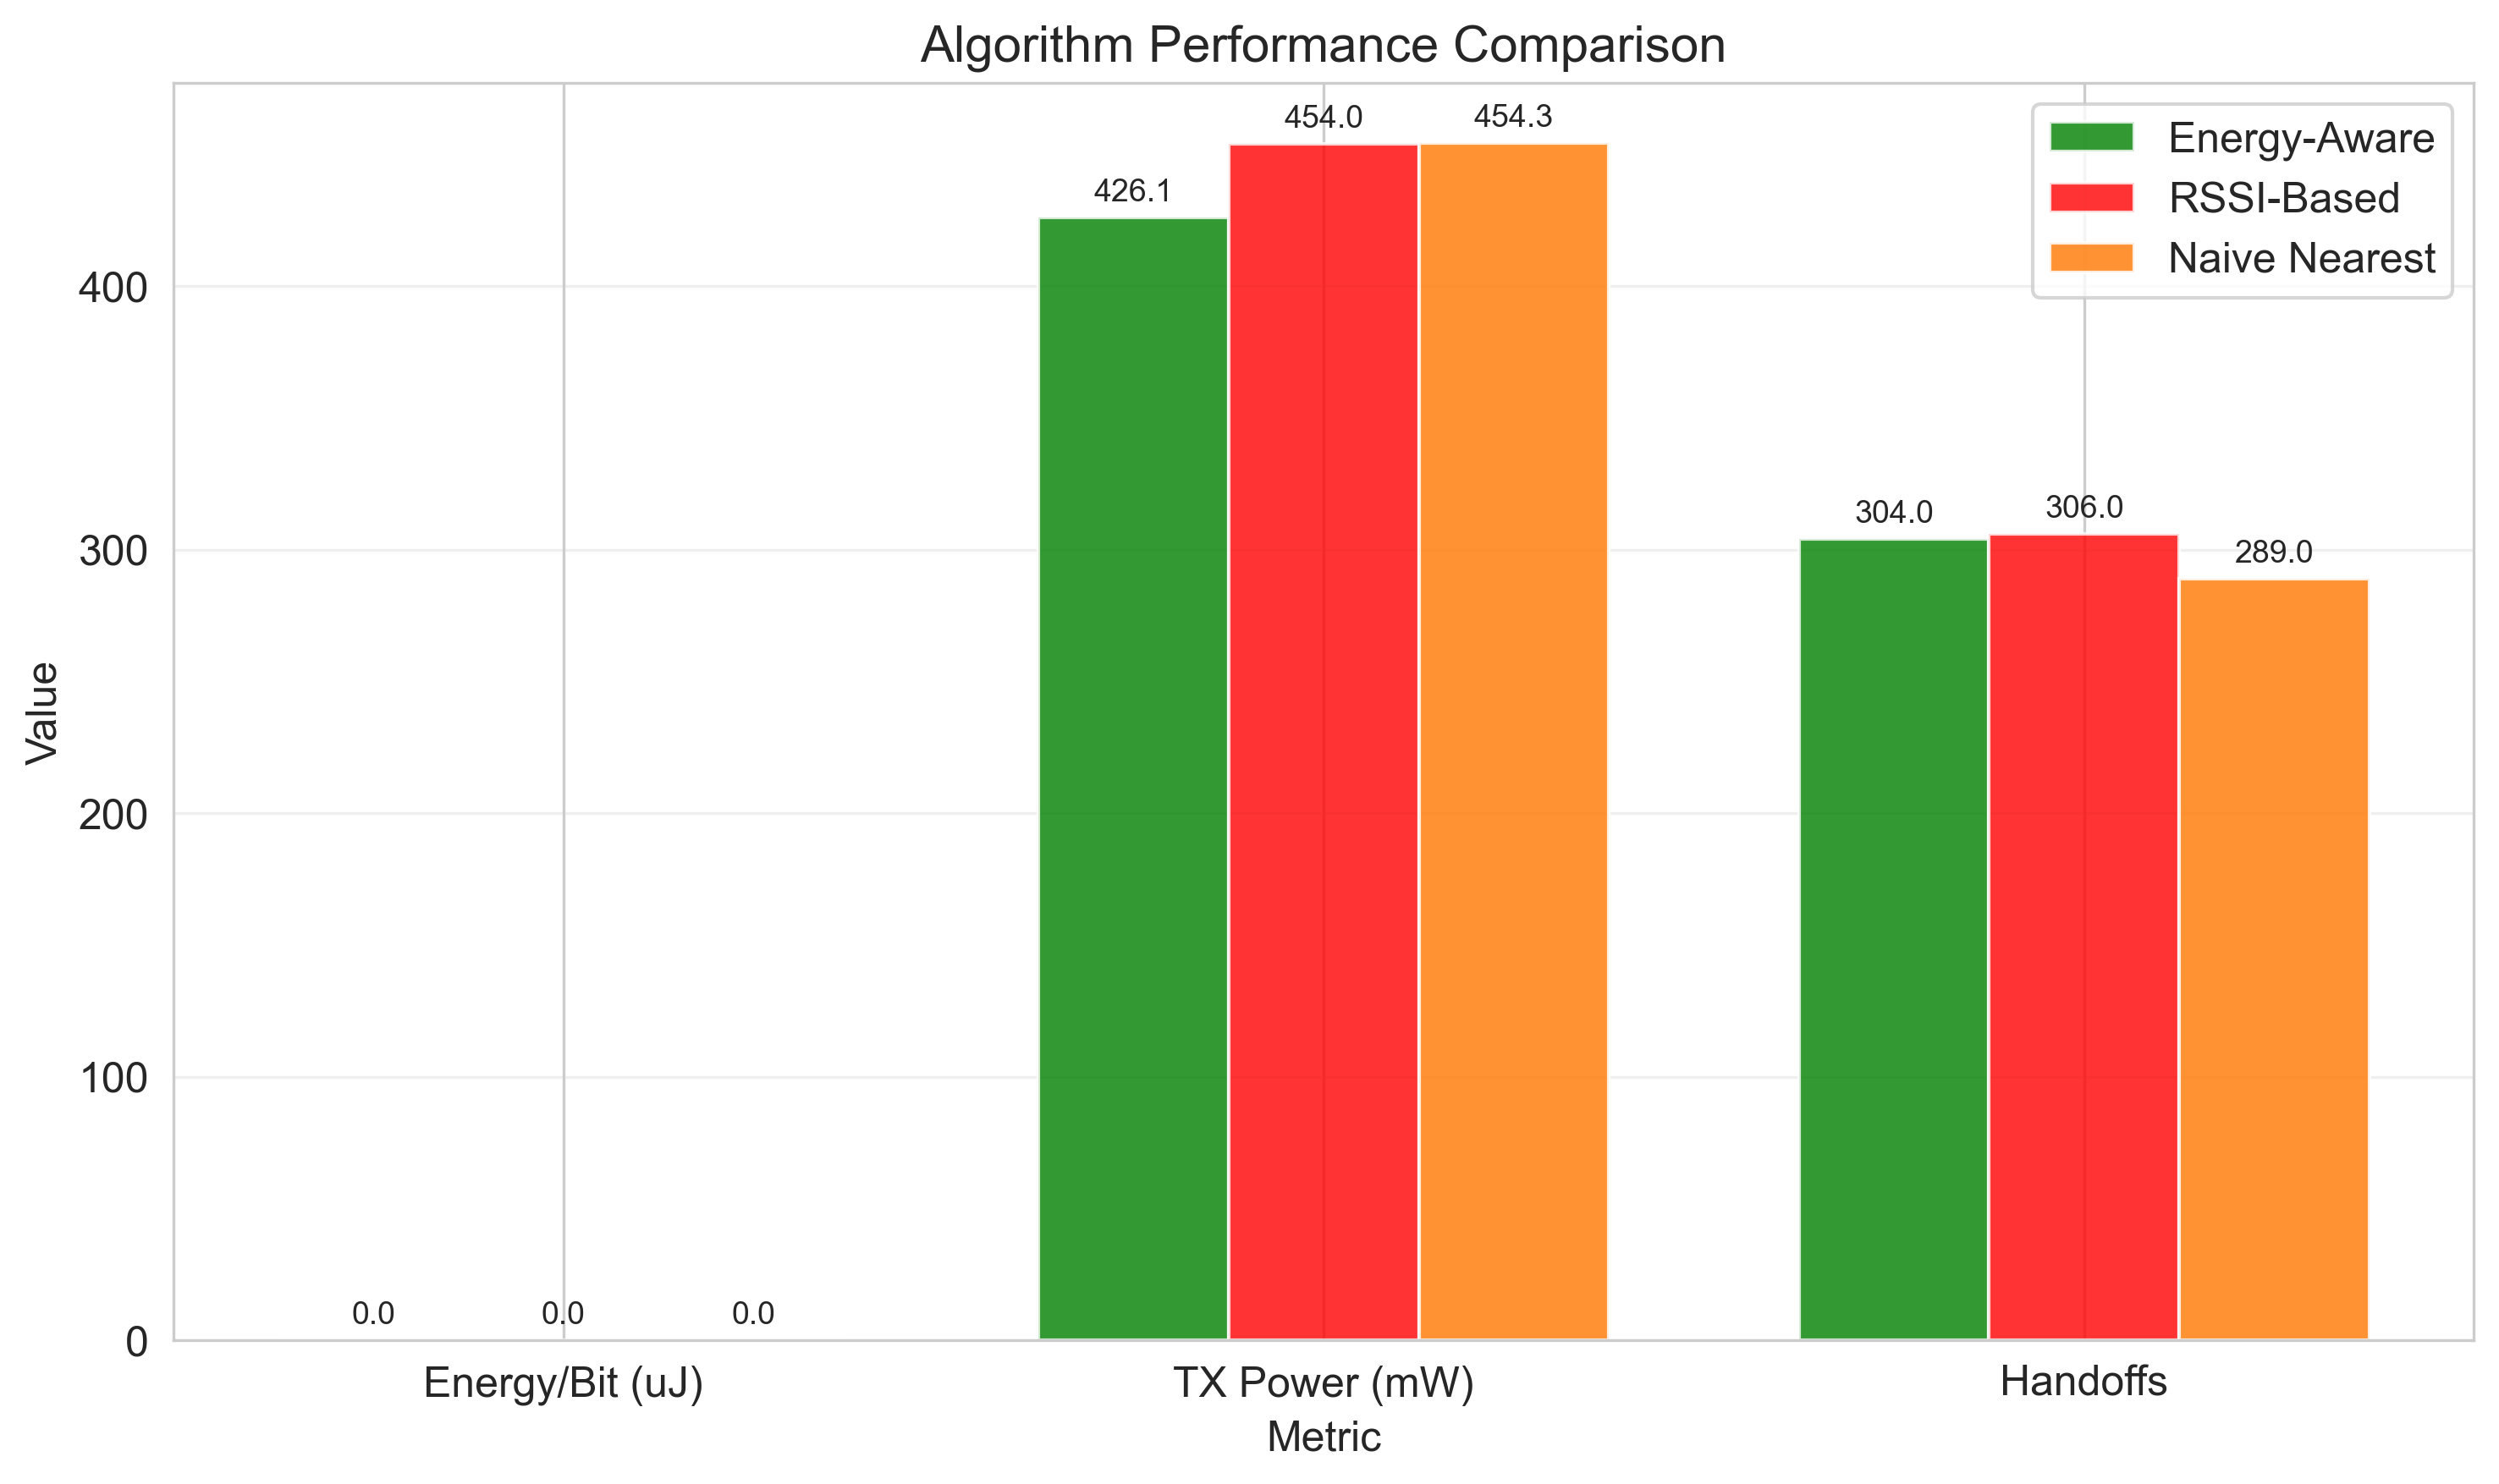
\includegraphics[
      width=\linewidth,
      height=0.13\textheight,
      keepaspectratio
    ]{results/bar_comparison.png}
  \end{minipage}\hfill
  \begin{minipage}[t]{0.47\linewidth}
    \centering
    \footnotesize
    \setlength{\tabcolsep}{2.5pt}
    \renewcommand{\arraystretch}{0.9}
    \begin{tabular}{@{}>{\raggedright\arraybackslash}p{0.4\linewidth}cc@{}}
      \toprule
      \textbf{Algorithm} & \textbf{Avg.\ EPB} & \textbf{Outage} \\
       & \textbf{(J/bit)} & \textbf{(\%)} \\
      \midrule
      \textbf{EAH (Proposed)} & $\mathbf{3.61\times10^{-8}}$ & \textbf{16.37} \\
      RSSI & $4.30\times10^{-8}$ & 22.75 \\
      SINR & $4.14\times10^{-8}$ & $\sim$21.0 \\
      Load-Aware RSSI & $4.31\times10^{-8}$ & $\sim$23.0 \\
      Naive Nearest & $3.66\times10^{-8}$ & $\sim$18.0 \\
      Literature UL-HO & $4.31\times10^{-8}$ & 24.75 \\
      LB-Aware RSRP & $4.34\times10^{-8}$ & $\sim$23.0 \\
      MDPI Energy Efficient & $5.18\times10^{-8}$ & 68.25 \\
      \bottomrule
    \end{tabular}\\[1pt]
    {\scriptsize 15-seed average; \textbf{bold} = best.}
  \end{minipage}
  \caption{(\textbf{Left})~Mean Energy Per Bit (EPB) comparison across all eight handoff
           algorithms (15-seed average, highway scenario, clear weather).
           (\textbf{Right})~Mean EPB and outage by algorithm; EAH achieves the lowest EPB
           while maintaining service quality superior to all baselines.}
\end{figure}

Across 15 independent simulation seeds (20 vehicles, 16 BSs, 1{,}200\,s, clear weather),
EAH achieves a mean EPB saving of \textbf{15.26\,\%\,$\pm$\,1.07\,\%} over RSSI
($p \approx 10^{-18}$, paired $t$-test) and a total energy saving of
\textbf{9.09\,\%\,$\pm$\,0.55\,\%}, directly reducing CO\textsubscript{2} by the same
margin. As shown in Fig.\,1, EAH records the lowest EPB among all algorithms
while simultaneously achieving the best outage probability (16.37\,\%) and highest mean
throughput (24.27\,Mbps). Handoff count falls by \textbf{20.52\,\%} and ping-pong rate
drops from 34.54\,\% to 20.46\,\%. The MDPI-inspired baseline achieves very few handoffs
but suffers severe service collapse (outage 68.25\,\%, throughput 8.29\,Mbps), confirming
that minimising switching alone does not produce a quality link. Scalability tests
(20--200 vehicles) show \textbf{$\approx$23\,\%} stable savings, and weather sweeps reveal
amplified gains under adverse conditions --- heavy rain \textbf{49\,\%}, thunderstorm
\textbf{69\,\%} --- precisely when energy-blind policies waste the most power.

These results demonstrate that handoff policy is an effective and largely untapped lever
for green vehicular networking. By explicitly minimising EPB rather than maximising signal
strength, EAH simultaneously reduces radio energy consumption, lowers CO\textsubscript{2}
emissions, and improves service reliability --- without any hardware modification. The
findings are directly relevant to sustainable transportation and climate-resilient smart-city
infrastructure, contributing to global efforts to reduce the carbon footprint of wireless
communication systems.

\vspace{2pt}
\hrule
\vspace{2pt}

% ---------- KEYWORDS ----------
\noindent\textbf{Keywords:}
V2X Communication;\;
Energy-Aware Handoff;\;
Green Wireless Networks;\;
CO\textsubscript{2} Reduction;\;
Sustainable Transportation

\end{document}
% ============================================================
